\documentclass{article}
\usepackage{graphicx} % Required for inserting images
\usepackage{biblatex}
\usepackage{indentfirst}
\usepackage{xcolor} 
\usepackage{parskip} 
\usepackage{subcaption}
\usepackage{placeins}
\usepackage{fourier} 
\usepackage{array}
\usepackage{makecell}
\usepackage[colorlinks]{hyperref}

\addbibresource{Bibliography.bib} 

\title{MFEM: A Modular Finite Element Methods Library}
\author{Elvin Gültekinoğlu }
\date{October 2023}

\begin{document}

\maketitle

\section{The Motivation Behind This Paper}
This document is prepared to summarize the key points of the article which is named as "MFEM: A Modular Finite Element Methods Library" and published in 2021. Throughout the text, the main points are highlighted and expressed with equations, figures and tables. 

\section{Abstract}
In R. Anderson, J. Andrej, A. Barker et al \cite{anderson2021mfem} MFEM is a C++ based library which is used for modular finite element methods related to arbitrary high-order finite element meshes and spaces and similar approaches. It becomes prominent with the fact that it is open-source, lightweight, flexible and scalable, which makes it easily accessible, portable and suitable for high-performance computing operations. Considering all these advantages, researchers are able to test their algorithms in settings which are high-order, parallel and GPU-accelerated. This paper is focused on the utilization of this library with theoretical background, explanations and applications. 

\section{Introduction}
Finite Element Method (FEM) is used to approximate the solutions of partial differential equations (PDE). It is mainly a discretization technique that utilizes unstructured grids. MFEM provides a support for these techniques and it is widely used due to its certain advantages. Also, being an open-source library, its source code is easily accessible on Spack, OpenHPC, and Github. 

MFEM offers certain advantages which makes it distinguisable from other similar packages used for FEM. These advantages come from its usability, accessibility and HPC efficiency. It also enables other researchers or scientists to contribute easily. With its positive features, MFEM is used in different general fields such as manufacturing, hydrodynamics, heat transfer, propulsion and paralellization. 

MFEM provides support for different type of meshes, solvers and numerical methods. In addition to these, it is utilizable for Message Passing Interface (MPI)-based paralellism, GPU acceleration with CUDA, OCCA, RAJA and OpenMP. 
\label{section_3}

\section{Theoretical Background}
In this section, general overview about the theory behind FEM and MFEM library is provided with mathematical expressions and related figures. 
\subsection{Finite Element Abstractions}
In order to use MFEM to solve related problems, there are certain classes, sub-classes, object types and functions which are used to implement a specific method according to the needs of the problem. To show this process, an example case can be considered, which is the model Poisson problem with homogeneous boundary conditions. The problem is defined as follows:\par 
Find u : $\Omega$ → R such that \par
-$\Delta$u = f in $\Omega$ \par
The approximate solution is obtained by solving the FEM problem with the given mesh. The problem is reduced to the following integral:
\begin{equation}
    \int_{\Omega}^{} \nabla u_h \nabla v_h = \int_{\Omega}^{} f v_h
    \label{equation_1}
\end{equation}
This integral is manupilated by defining basis function $\phi$ for the related space $V_h$ and the Equation \ref{equation_1} is rewritten. For the rewritten version, see the Equation \ref{equation_3}. By calling necessary methods from revelant classes and methods, the solution is obtained. 
\begin{equation}
    \Sigma_{j=0} c_j \int_{\Omega}^{} \nabla \phi \nabla \phi = \int_{\Omega}^{} f \phi
    \label{equation_3}
\end{equation}

\subsection{Meshes}
As mentioned in Section \ref{section_3} MFEM is used for different type of meshes such as triangular, quadrilateral, tetrahedral, hexahedral and prismatic. Considering these types, there are two main classes available for meshes in the software. These are "Mesh" and "ParMesh" classes. The former one is used for a serial mesh and the latter one is used for an MPI-distributed parallel mesh.
\subsubsection{The Types of Meshes}
Serial, unstructured conforming mesh in MFEM is described in terms of two different parts: topological (connectivity) data and geometric (coordinates) data. Topological part is mainly about the type, attribute, vertex indices, edges, faces and connection elements of meshes. Geometric part describes the aspects related to spatial features of meshes such as coordinates of vertices.  
To define the precise shape of a mesh element, mapping is performed. This process is presented in the Figure \ref{figure_1}. The driving equation behind this mapping operation is given in the Equation \ref{equation_2} . 
\begin{figure}[hbt!]
    \centering
    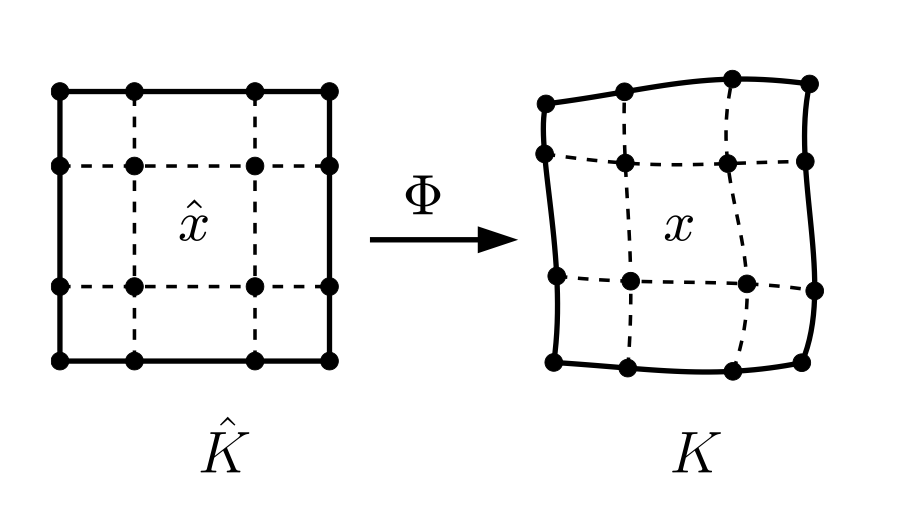
\includegraphics[width=0.5\textwidth]{Figures/Figure_1.png}
    \caption{The mapping of an element from the reference element to bi-cubic element in K physical space with high-order nodes.}
    \label{figure_1}
\end{figure}
\begin{equation}
    \Omega(x) = \Sigma_{i=1}^N x_{K_i} w(x) 
    \label{equation_2}
\end{equation} \par
Other types of meshes are non-conforming meshes which are defined as conforming meshes with additional constraints, NURBS meshes used in geometric modeling mainly and parallel meshes for MPI-based applications. 
\section{High Performance Computing}
In this section, high performance computing feature of MFEM is examined.
\subsection{Parallel Meshes}
MFEM is a proper software to be used in applications involving large scale parallelism with Message Passing Interface (MPI). In parallel solving, the problem is analyzed in pieces after it is decomposed into K different parts. As an example case, solution of a Poisson problem is given in the Figure \ref{figure_2}. 
\begin{figure}[hbt!]
\centering
\begin{subfigure}{0.4\textwidth}
    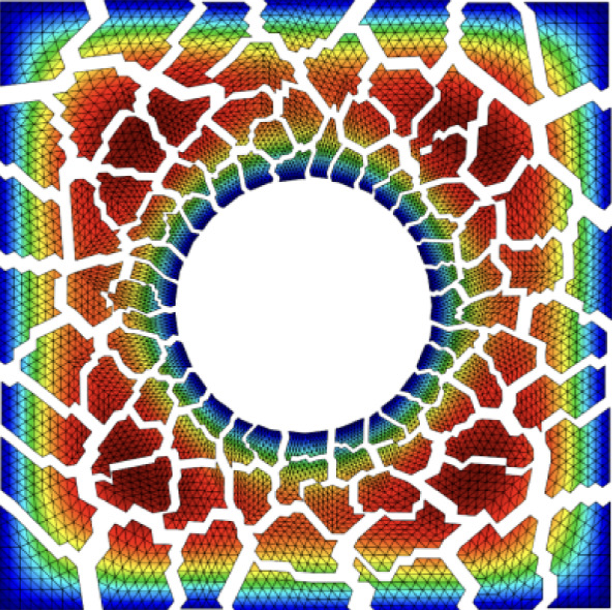
\includegraphics[width=\textwidth]{Figures/Figure_2_1.png}
\end{subfigure}
\hfill
\begin{subfigure}{0.4\textwidth}
    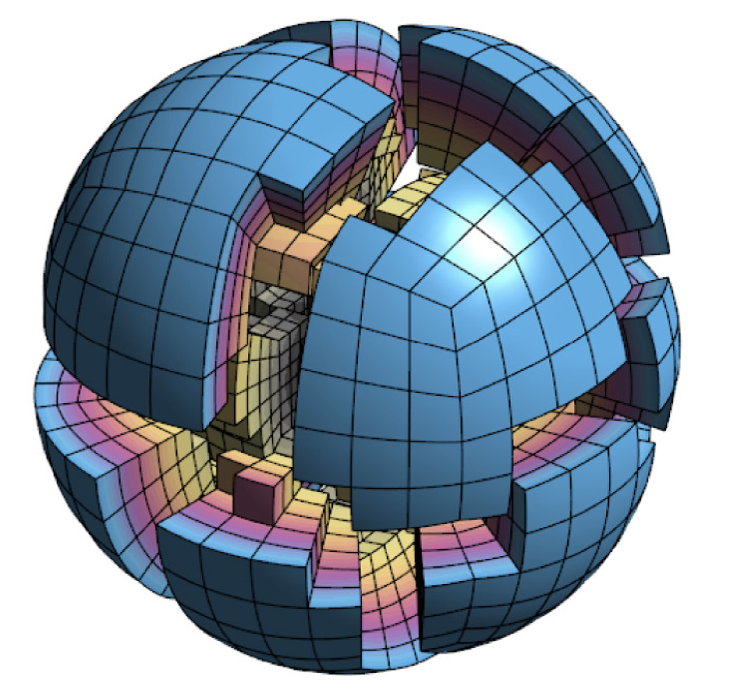
\includegraphics[width=\textwidth]{Figures/Figure_2_2.png}
\end{subfigure}
\caption{Left: Solving a Poisson problem in parallel on 100 processors. Right: Unstructured parallel decomposition of a fourth order NURBS mesh of the unit ball on 16 processors.}
\label{figure_2}
\end{figure}
\FloatBarrier
\subsection{GPU Acceleration}
With the release of version of 4.0 MFEM, the compatibility with hardware accelerators is also announced, which amounts to the opportunity of using GPUs and libraries such as CUDA, OCCA, libCEED, RAJA and OpenMP. This feature leads to certain advantages. One main advantage of MFEM about this is being able to select backends at runtime so as to increase performance. MFEM achieves this by its modular design for accelerator support which is given in the Figure \ref{figure_3}. 
\begin{figure}[hbt!]
    \centering
    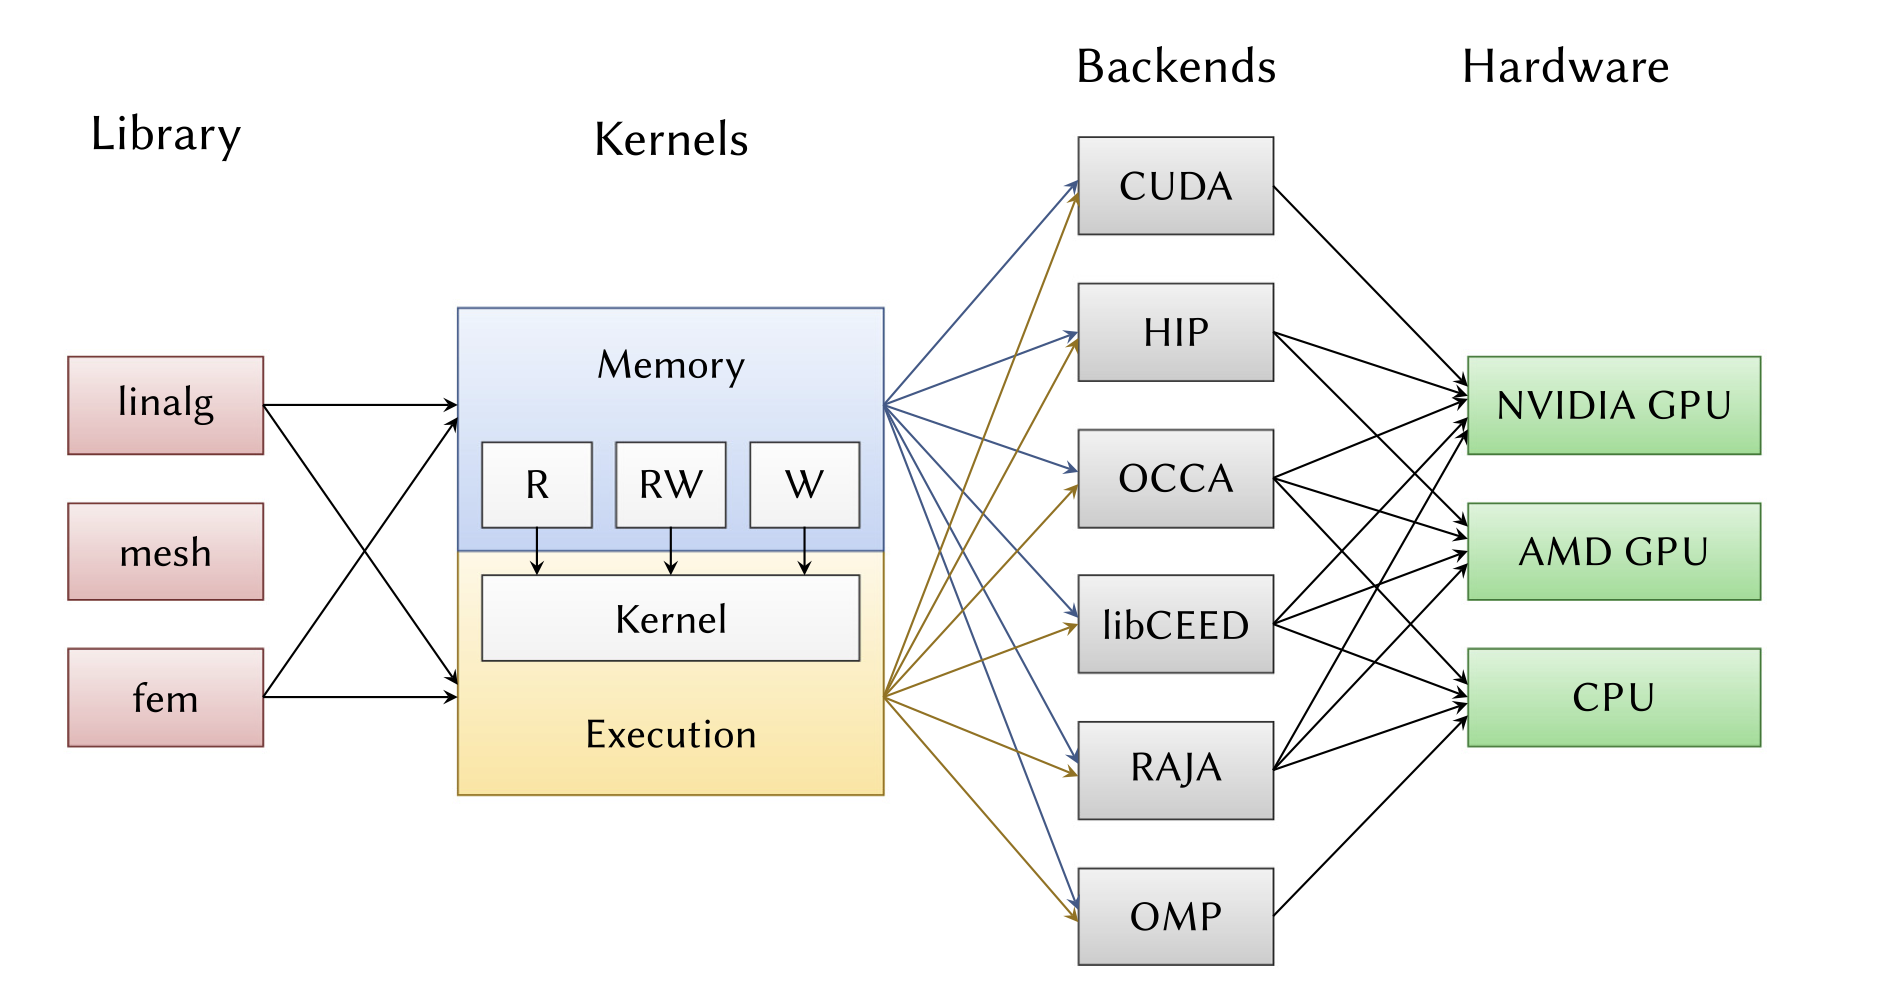
\includegraphics[width=1.0\textwidth]{Figures/Figure_3.png}
    \caption{Diagram of MFEM’s modular design for accelerator support. }
    \label{figure_3}
\end{figure}
\\In order to evaluate the performance of aforementioned aspects, performance tests are conducted. These tests are performed on a Linux-based computer with GPU, multi-core and CPU along with different libraries. As a result, it is observed that GPU acceleration has a positive effect on performance. Test results are provided in the Table \ref{table_1}. 
\begin{table}[hbt!]
    \begin{center}
    \begin{tabular}{ ||c c c c|| } 
         \hline
          &  & p=1 & p=2  \\
         \hline\hline
         GPU & \thead{OCCA-CUDA\\ RAJA-CUDA\\ CUDA\\ CEED-CUDA} & \thead{0.52 \\ 0.38 \\ 0.36 \\ 0.19} & \thead{0.31\\ 0.30\\ 0.26\\ 0.15} \\ 
         \hline
         Multicore & \thead{OCCA-OMP\\ RAJA-OMP\\ OMP\\ MPI} & \thead{3.34 \\ 3.32 \\ 3.30 \\ 2.72} & \thead{2.41 \\ 2.45 \\ 2.46 \\ 1.66}\\ 
         \hline
         CPU & \thead{OCCA-CPU\\ RAJA-CPU\\ CPU\\ CEED-AVX\\ CEED-XSMM} & \thead{21.05\\ 45.42\\ 25.18\\ 43.04\\ 53.80} & \thead{15.77\\ 16.53\\ 16.11\\ 18.16\\ 20.13} \\ 
         \hline
     \end{tabular}
    \caption{Performance results with MFEM-4.0}
    \label{table_1}
    \end{center}
\end{table}
\FloatBarrier
\section{Conclusion}
In this paper, MFEM library is introduced with its characteristics, algorithms, advantages and applications as a summary. MFEM is getting more and more popular these days among scientists and researchers because of its easiness and accessibility as well as high performance capability. 
\printbibliography
\end{document}
